\section{Logistic regression (ordinal/nominal response)}
\frame{\sectionpage}


\begin{frame}{Logistic regression}

  \begin{itemize}
  \item When response variable is measured/counted, regression can work well.
  \item But what if response is yes/no, lived/died, success/failure?
  \item Model {\em probability} of success.
  \item Probability must be between 0 and 1; need method that ensures this.
  \item {\em Logistic regression} does this. In R, is a
    \emph{generalized linear model} with binomial ``family'': 
\texttt{glm(y\textasciitilde x,family="binomial")}
    
  \item Begin with simplest case.
    
  \end{itemize}
  
\end{frame}

\begin{frame}[fragile]{The rats, part 1}

  \begin{itemize}
  \item Rats given dose of some poison; either live or die:

{\scriptsize
\begin{verbatim}
dose status
0 lived
1 died
2 lived
3 lived
4 died
5 died
\end{verbatim}
}
\item Basic logistic regression analysis:

{\footnotesize
 
\begin{knitrout}
\definecolor{shadecolor}{rgb}{0.969, 0.969, 0.969}\color{fgcolor}\begin{kframe}
\begin{alltt}
\hlstd{rats}\hlkwb{=}\hlkwd{read.table}\hlstd{(}\hlstr{"rat.txt"}\hlstd{,}\hlkwc{header}\hlstd{=T)}
\hlstd{rats}
\end{alltt}
\begin{verbatim}
##   dose status
## 1    0  lived
## 2    1   died
## 3    2  lived
## 4    3  lived
## 5    4   died
## 6    5   died
\end{verbatim}
\begin{alltt}
\hlkwd{attach}\hlstd{(rats)}
\hlstd{rats.1}\hlkwb{=}\hlkwd{glm}\hlstd{(status}\hlopt{~}\hlstd{dose,}\hlkwc{family}\hlstd{=}\hlstr{"binomial"}\hlstd{)}
\end{alltt}
\end{kframe}
\end{knitrout}
}
  

  \end{itemize}
  



\end{frame}
  

\begin{frame}[fragile]{Output}

  {\footnotesize
 
\begin{knitrout}
\definecolor{shadecolor}{rgb}{0.969, 0.969, 0.969}\color{fgcolor}\begin{kframe}
\begin{alltt}
\hlkwd{summary}\hlstd{(rats.1)}
\end{alltt}
\begin{verbatim}
## 
## Call:
## glm(formula = status ~ dose, family = "binomial")
## 
## Deviance Residuals: 
##       1        2        3        4        5        6  
##  0.5835  -1.6254   1.0381   1.3234  -0.7880  -0.5835  
## 
## Coefficients:
##             Estimate Std. Error z value Pr(>|z|)
## (Intercept)   1.6841     1.7979   0.937    0.349
## dose         -0.6736     0.6140  -1.097    0.273
## 
## (Dispersion parameter for binomial family taken to be 1)
## 
##     Null deviance: 8.3178  on 5  degrees of freedom
## Residual deviance: 6.7728  on 4  degrees of freedom
## AIC: 10.773
## 
## Number of Fisher Scoring iterations: 4
\end{verbatim}
\end{kframe}
\end{knitrout}
}   

\end{frame}


\begin{frame}{Interpreting the output}
  \begin{itemize}
  \item Like (multiple) regression, get
   tests of significance of individual $x$'s
  \item     Here not significant (only 6 observations).
  \item ``Slope'' for dose is negative, meaning that as dose increases, probability of event modelled (survival) decreases.

\end{itemize}

\end{frame}

\begin{frame}[fragile]{Output part 2: predicted survival probs}

  
 
\begin{knitrout}
\definecolor{shadecolor}{rgb}{0.969, 0.969, 0.969}\color{fgcolor}\begin{kframe}
\begin{alltt}
\hlstd{p}\hlkwb{=}\hlkwd{predict}\hlstd{(rats.1,}\hlkwc{type}\hlstd{=}\hlstr{"response"}\hlstd{)}
\hlkwd{cbind}\hlstd{(rats,p)}
\end{alltt}
\begin{verbatim}
##   dose status         p
## 1    0  lived 0.8434490
## 2    1   died 0.7331122
## 3    2  lived 0.5834187
## 4    3  lived 0.4165813
## 5    4   died 0.2668878
## 6    5   died 0.1565510
\end{verbatim}
\end{kframe}
\end{knitrout}
  
\end{frame}




\begin{frame}[fragile]{The rats, more}

  \begin{itemize}
  \item More realistic: more rats at each dose (say 10).
  \item Listing each rat on one line makes a big data file.
  \item Use format below: dose, number of survivals, number of deaths.
\begin{verbatim}
dose lived died
   0    10    0
   1     7    3 
   2     6    4 
   3     4    6 
   4     2    8 
   5     1    9  
\end{verbatim}


  \item 6 lines of data correspond to 60 actual rats.

  \item Saved in \texttt{rat2.txt}.

  \end{itemize}
  
\end{frame}

\begin{frame}[fragile]{Code for this logistic regression}

 
\begin{knitrout}
\definecolor{shadecolor}{rgb}{0.969, 0.969, 0.969}\color{fgcolor}\begin{kframe}
\begin{alltt}
\hlkwd{detach}\hlstd{(rats)}
\hlstd{rat2}\hlkwb{=}\hlkwd{read.table}\hlstd{(}\hlstr{"rat2.txt"}\hlstd{,}\hlkwc{header}\hlstd{=T)}
\hlstd{rat2}
\end{alltt}
\begin{verbatim}
##   dose lived died
## 1    0    10    0
## 2    1     7    3
## 3    2     6    4
## 4    3     4    6
## 5    4     2    8
## 6    5     1    9
\end{verbatim}
\begin{alltt}
\hlkwd{attach}\hlstd{(rat2)}
\hlstd{response}\hlkwb{=}\hlkwd{cbind}\hlstd{(lived,died)}
\hlstd{rat2.1}\hlkwb{=}\hlkwd{glm}\hlstd{(response}\hlopt{~}\hlstd{dose,}\hlkwc{family}\hlstd{=}\hlstr{"binomial"}\hlstd{)}
\end{alltt}
\end{kframe}
\end{knitrout}
  
\begin{itemize}
\item Note construction of \emph{two-column} response, \#survivals in
  first column, \#deaths in second.
\end{itemize}


  
\end{frame}

\begin{frame}[fragile]{Output}

{\footnotesize  
 
\begin{knitrout}
\definecolor{shadecolor}{rgb}{0.969, 0.969, 0.969}\color{fgcolor}\begin{kframe}
\begin{alltt}
\hlkwd{summary}\hlstd{(rat2.1)}
\end{alltt}
\begin{verbatim}
## 
## Call:
## glm(formula = response ~ dose, family = "binomial")
## 
## Deviance Residuals: 
##       1        2        3        4        5        6  
##  1.3421  -0.7916  -0.1034   0.1034   0.0389   0.1529  
## 
## Coefficients:
##             Estimate Std. Error z value Pr(>|z|)    
## (Intercept)   2.3619     0.6719   3.515 0.000439 ***
## dose         -0.9448     0.2351  -4.018 5.87e-05 ***
## ---
## Signif. codes:  0 '***' 0.001 '**' 0.01 '*' 0.05 '.' 0.1 ' ' 1
## 
## (Dispersion parameter for binomial family taken to be 1)
## 
##     Null deviance: 27.530  on 5  degrees of freedom
## Residual deviance:  2.474  on 4  degrees of freedom
## AIC: 18.94
## 
## Number of Fisher Scoring iterations: 4
\end{verbatim}
\end{kframe}
\end{knitrout}
}
  

\end{frame}

\begin{frame}[fragile]{Predicted survival probs}

 
\begin{knitrout}
\definecolor{shadecolor}{rgb}{0.969, 0.969, 0.969}\color{fgcolor}\begin{kframe}
\begin{alltt}
\hlstd{p}\hlkwb{=}\hlkwd{predict}\hlstd{(rat2.1,}\hlkwc{type}\hlstd{=}\hlstr{"response"}\hlstd{)}
\hlkwd{cbind}\hlstd{(rat2,p)}
\end{alltt}
\begin{verbatim}
##   dose lived died         p
## 1    0    10    0 0.9138762
## 2    1     7    3 0.8048905
## 3    2     6    4 0.6159474
## 4    3     4    6 0.3840526
## 5    4     2    8 0.1951095
## 6    5     1    9 0.0861238
\end{verbatim}
\end{kframe}
\end{knitrout}
  
  

  
\end{frame}

\begin{frame}[fragile]{Comments}

\begin{itemize}
\item Significant effect of dose. 
\item Effect of larger dose is to decrease survival probability
  (``slope'' negative; also see in decreasing predictions.)
\end{itemize}
  
\end{frame}


\begin{frame}{Multiple logistic regression}

  \begin{itemize}
  \item With more than one $x$, works much like multiple regression.
  \item Example: study of patients with blood poisoning severe enough to warrant surgery. Relate survival to other potential risk factors.
  \item Variables, 1=present, 0=absent:
    \begin{itemize}
    \item survival (death from sepsis=1), response
    \item shock
    \item malnutrition
    \item alcoholism
    \item age (as numerical variable)
    \item bowel infarction
    \end{itemize}
  \item See what relates to death.
  \end{itemize}


  
\end{frame}

\begin{frame}[fragile]{Read in data and fit model}

 
\begin{knitrout}
\definecolor{shadecolor}{rgb}{0.969, 0.969, 0.969}\color{fgcolor}\begin{kframe}
\begin{alltt}
\hlkwd{detach}\hlstd{(rat2)}
\hlstd{sepsis}\hlkwb{=}\hlkwd{read.table}\hlstd{(}\hlstr{"sepsis.txt"}\hlstd{,}\hlkwc{header}\hlstd{=T)}
\hlkwd{head}\hlstd{(sepsis)}
\end{alltt}
\begin{verbatim}
##   death shock malnut alcohol age bowelinf
## 1     0     0      0       0  56        0
## 2     0     0      0       0  80        0
## 3     0     0      0       0  61        0
## 4     0     0      0       0  26        0
## 5     0     0      0       0  53        0
## 6     1     0      1       0  87        0
\end{verbatim}
\begin{alltt}
\hlkwd{attach}\hlstd{(sepsis)}
\hlstd{sepsis.1}\hlkwb{=}\hlkwd{glm}\hlstd{(death}\hlopt{~}\hlstd{shock}\hlopt{+}\hlstd{malnut}\hlopt{+}\hlstd{alcohol}\hlopt{+}\hlstd{age}\hlopt{+}
              \hlstd{bowelinf,}\hlkwc{family}\hlstd{=}\hlstr{"binomial"}\hlstd{)}
\end{alltt}
\end{kframe}
\end{knitrout}
  

\end{frame}

\begin{frame}[fragile]{Output part 1}

 
\begin{knitrout}
\definecolor{shadecolor}{rgb}{0.969, 0.969, 0.969}\color{fgcolor}\begin{kframe}
\begin{alltt}
\hlkwd{summary}\hlstd{(sepsis.1)}\hlopt{$}\hlstd{coefficients}
\end{alltt}
\begin{verbatim}
##                Estimate Std. Error   z value     Pr(>|z|)
## (Intercept) -9.75390560 2.54169523 -3.837559 0.0001242633
## shock        3.67386585 1.16481138  3.154044 0.0016102504
## malnut       1.21658106 0.72822359  1.670615 0.0947978002
## alcohol      3.35488462 0.98210260  3.416023 0.0006354299
## age          0.09215268 0.03032368  3.038968 0.0023739015
## bowelinf     2.79758637 1.16397170  2.403483 0.0162397151
\end{verbatim}
\end{kframe}
\end{knitrout}
%$

\begin{itemize}
\item All P-values fairly small
\item but \texttt{malnut} not significant: remove.
\end{itemize}


\end{frame}

\begin{frame}[fragile]{Removing \texttt{malnut}}

 
\begin{knitrout}
\definecolor{shadecolor}{rgb}{0.969, 0.969, 0.969}\color{fgcolor}\begin{kframe}
\begin{alltt}
\hlstd{sepsis.2}\hlkwb{=}\hlkwd{glm}\hlstd{(death}\hlopt{~}\hlstd{shock}\hlopt{+}\hlstd{alcohol}\hlopt{+}\hlstd{age}\hlopt{+}
              \hlstd{bowelinf,}\hlkwc{family}\hlstd{=}\hlstr{"binomial"}\hlstd{)}
\hlkwd{summary}\hlstd{(sepsis.2)}\hlopt{$}\hlstd{coefficients}
\end{alltt}
\begin{verbatim}
##                Estimate Std. Error   z value     Pr(>|z|)
## (Intercept) -8.89458992 2.31689479 -3.839013 0.0001235297
## shock        3.70119321 1.10353465  3.353944 0.0007966854
## alcohol      3.18590397 0.91724569  3.473338 0.0005140283
## age          0.08983175 0.02921528  3.074821 0.0021062897
## bowelinf     2.38646847 1.07226618  2.225631 0.0260389310
\end{verbatim}
\end{kframe}
\end{knitrout}

\begin{itemize}
\item Everything significant now.
\end{itemize}
  
 
  
\end{frame}

\begin{frame}[fragile]{Comments}

%$  
  \begin{itemize}
\item Most of the original $x$'s helped predict death. Only \texttt{malnut} seemed not to add anything.
\item Removed \texttt{malnut} and tried again.
\item Everything remaining is significant (though \texttt{bowelinf}
  actually became \emph{less} significant).
\item All coefficients are \emph{positive}, so having any of the risk
  factors (or being older)
  \emph{increases} risk of death.  
\end{itemize}

\end{frame}

\begin{frame}[fragile]{Predictions from model without ``malnut''}
  
  \begin{itemize}
  \item A few chosen at random. Define vector containing rows you
    want, then pick out of data frame and predictions:

    {\small
\begin{knitrout}
\definecolor{shadecolor}{rgb}{0.969, 0.969, 0.969}\color{fgcolor}\begin{kframe}
\begin{alltt}
\hlstd{sepsis.pred}\hlkwb{=}\hlkwd{predict}\hlstd{(sepsis.2,}\hlkwc{type}\hlstd{=}\hlstr{"response"}\hlstd{)}
\hlstd{myrows}\hlkwb{=}\hlkwd{c}\hlstd{(}\hlnum{4}\hlstd{,}\hlnum{1}\hlstd{,}\hlnum{2}\hlstd{,}\hlnum{11}\hlstd{,}\hlnum{32}\hlstd{)}
\hlkwd{cbind}\hlstd{(sepsis[myrows,],}\hlkwc{p}\hlstd{=sepsis.pred[myrows])}
\end{alltt}
\begin{verbatim}
##    death shock malnut alcohol age bowelinf           p
## 4      0     0      0       0  26        0 0.001415347
## 1      0     0      0       0  56        0 0.020552383
## 2      0     0      0       0  80        0 0.153416834
## 11     1     0      0       1  66        1 0.931290137
## 32     1     0      0       1  49        0 0.213000997
\end{verbatim}
\end{kframe}
\end{knitrout}
}

\item Survival chances pretty good if no risk factors, though decreasing with age.
\item Having more than one risk factor reduces survival chances dramatically.
\item Usually model does a good job of predicting survival, but occasionally someone dies who was predicted to survive.
  \end{itemize}
  
\end{frame}

\begin{frame}[fragile]{Assessing proportionality of odds for age}
  \begin{itemize}
  \item An assumption we made is that log-odds of survival depends
    linearly on age.
  \item Hard to get your head around, but 
    basic idea is that survival chances go continuously up (or down)
    with age, instead of (for example) going up and then down.
  \item In this case, seems reasonable, but should check:

\begin{knitrout}
\definecolor{shadecolor}{rgb}{0.969, 0.969, 0.969}\color{fgcolor}\begin{kframe}
\begin{alltt}
\hlkwd{library}\hlstd{(tidyverse)}
\end{alltt}


{\ttfamily\noindent\itshape\color{messagecolor}{\#\# Loading tidyverse: ggplot2\\\#\# Loading tidyverse: tibble\\\#\# Loading tidyverse: tidyr\\\#\# Loading tidyverse: readr\\\#\# Loading tidyverse: purrr\\\#\# Loading tidyverse: dplyr}}

{\ttfamily\noindent\itshape\color{messagecolor}{\#\# Conflicts with tidy packages ----------------------------------------------}}

{\ttfamily\noindent\itshape\color{messagecolor}{\#\# filter(): dplyr, stats\\\#\# lag():\ \ \ \ dplyr, stats}}\end{kframe}
\end{knitrout}
  \end{itemize}
    

\end{frame}
 

\begin{frame}[fragile]{Residuals vs.\ age}

 
\begin{knitrout}
\definecolor{shadecolor}{rgb}{0.969, 0.969, 0.969}\color{fgcolor}\begin{kframe}
\begin{alltt}
\hlstd{r}\hlkwb{=}\hlkwd{residuals}\hlstd{(sepsis.2)}
\hlkwd{ggplot}\hlstd{(sepsis,}\hlkwd{aes}\hlstd{(}\hlkwc{x}\hlstd{=age,}\hlkwc{y}\hlstd{=r))}\hlopt{+}\hlkwd{geom_point}\hlstd{()}
\end{alltt}
\end{kframe}
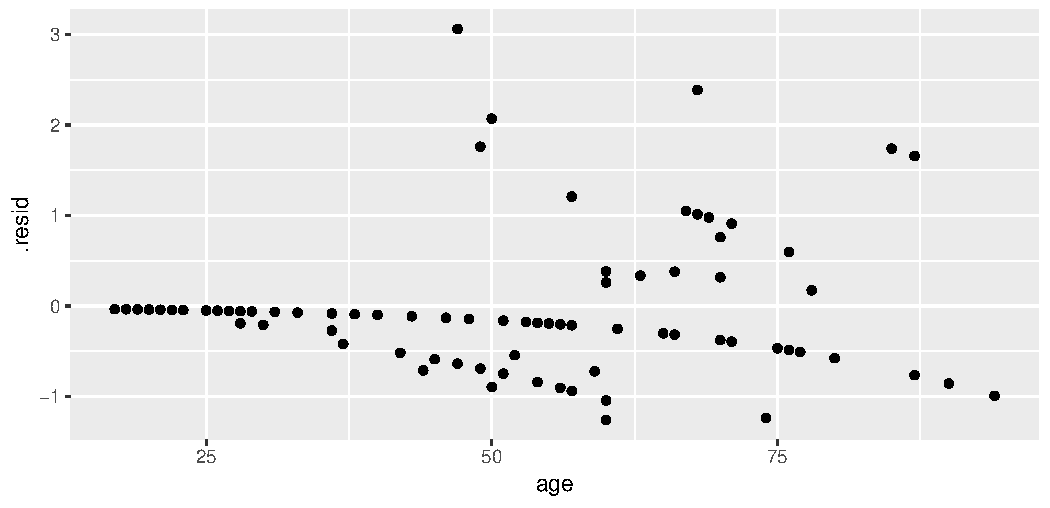
\includegraphics[width=\maxwidth]{figure/virtusentella-1} 

\end{knitrout}
  
  
\begin{itemize}
\item No apparent problems overall.
\item Confusing ``line'' across: no risk factors, survived. 
\end{itemize}
  
\end{frame}

\begin{frame}[fragile]{Probability and odds}
  
  \begin{itemize}
  \item For probability $p$, odds is $p/(1-p)$. Examples:
    \vfill
    \begin{tabular}{rrrl}
      \hline
      Prob.\ & Odds & log-odds & in words\\
      \hline
      0.5 & $0.5/0.5=1/1=1.00$ & 0.00 &  ``even money''\\
      0.1 & $0.1/0.9=1/9=0.11$ & $-2.20$ & ``9 to 1''\\
      0.4 & $0.4/0.6=1/1.5=0.67$ & $-0.41$ & ``1.5 to 1''\\
      0.8 & $0.8/0.2=4/1=4.00$ & 1.39 & ``4 to 1 on''\\
      \hline
    \end{tabular}
    \vfill
  \item Gamblers use odds: if you win at 9 to 1 odds, get original
    stake back plus 9 times the stake.
  \item Probability has to be between 0 and 1
  \item Odds between 0 and infinity
  \item \emph{Log}-odds can be anything: any log-odds corresponds to
    valid probability.
  \end{itemize}
  
\end{frame}

\begin{frame}[fragile]{Odds ratio}
  
  \begin{itemize}
  \item Suppose 90 of 100 men drank wine last week, but only 20 of 100 women.
  \item Prob of man drinking wine $90/100=0.9$, woman $20/100=0.2$.
  \item Odds of man drinking wine $0.9/0.1=9$, woman $0.2/0.8=0.25$.
  \item Ratio of odds is $9/0.25=36$.
  \item Way of quantifying difference between men and women: ``odds of
    drinking wine 36 times larger for males than females''. 
  \end{itemize}
  
\end{frame}

\begin{frame}[fragile]{Multiplying the odds}

  \begin{itemize}
  \item Can interpret slopes by taking ``exp'' of them. I ignore intercept.

 
\begin{knitrout}
\definecolor{shadecolor}{rgb}{0.969, 0.969, 0.969}\color{fgcolor}\begin{kframe}
\begin{alltt}
\hlstd{cc}\hlkwb{=}\hlkwd{exp}\hlstd{(}\hlkwd{coef}\hlstd{(sepsis.2)[}\hlopt{-}\hlnum{1}\hlstd{])}
\hlkwd{round}\hlstd{(cc,}\hlnum{2}\hlstd{)}
\end{alltt}
\begin{verbatim}
##    shock  alcohol      age bowelinf 
##    40.50    24.19     1.09    10.88
\end{verbatim}
\end{kframe}
\end{knitrout}

\item These say ``how much do you \emph{multiply} odds of death by
    for increase of 1 in corresponding risk factor?'' Or, what is odds
    ratio for that factor being 1 (present) vs.\ 0 (absent)?
  \item Eg.\ being alcoholic vs.\ not increases odds of death by 24 times
  \item One year older multiplies odds by about 1.1 times. Over 40 years,
    about  $1.09^{40}=31$ times. 
  \item Tidy up:
 
\begin{knitrout}
\definecolor{shadecolor}{rgb}{0.969, 0.969, 0.969}\color{fgcolor}\begin{kframe}
\begin{alltt}
\hlkwd{detach}\hlstd{(sepsis)}
\end{alltt}
\end{kframe}
\end{knitrout}
    

  \end{itemize}
  
\end{frame}

\begin{frame}[fragile]{Odds ratio and relative risk}
  
  \begin{itemize}
  \item \textbf{Relative risk} is ratio of probabilities.
  \item Above: 90 of 100 men (0.9) drank wine, 20 of 100 women (0.2).
  \item Relative risk 0.9/0.2=4.5. (odds ratio was 36).
  \item When probabilities small, relative risk and odds ratio similar.
  \item Eg.\ prob of man having disease 0.02, woman 0.01.
  \item Relative risk $0.02/0.01=2$.
  \item Odds for men and for women:
 
\begin{knitrout}
\definecolor{shadecolor}{rgb}{0.969, 0.969, 0.969}\color{fgcolor}\begin{kframe}
\begin{alltt}
\hlstd{(od1}\hlkwb{=}\hlnum{0.02}\hlopt{/}\hlnum{0.98}\hlstd{)}
\end{alltt}
\begin{verbatim}
## [1] 0.02040816
\end{verbatim}
\begin{alltt}
\hlstd{(od2}\hlkwb{=}\hlnum{0.01}\hlopt{/}\hlnum{0.99}\hlstd{)}
\end{alltt}
\begin{verbatim}
## [1] 0.01010101
\end{verbatim}
\end{kframe}
\end{knitrout}

\item Odds ratio 
 
\begin{knitrout}
\definecolor{shadecolor}{rgb}{0.969, 0.969, 0.969}\color{fgcolor}\begin{kframe}
\begin{alltt}
\hlstd{od1}\hlopt{/}\hlstd{od2} \hlcom{# very close to 2}
\end{alltt}
\begin{verbatim}
## [1] 2.020408
\end{verbatim}
\end{kframe}
\end{knitrout}
  
    
  \end{itemize}
  
\end{frame}



\begin{frame}{More than 2 response categories}

  \begin{itemize}
  \item With 2 response categories, model the probability of one, and prob of other is one minus that. So doesn't matter which category you model.
  \item With more than 2 categories, have to think more carefully about the categories: are they
    \begin{itemize}
    \item {\em ordered}: you can put them in a natural order (like low, medium, high)
    \item {\em nominal}: ordering the categories doesn't make sense (like red, green, blue).
    \end{itemize}
  \item R handles both kinds of response; learn how.
  \end{itemize}
  
\end{frame}

\begin{frame}[fragile]{Ordinal response: the miners}


  \begin{itemize}
  \item 
Model probability of being in given category {\em or lower}.
\item Example: coal-miners often suffer disease pneumoconiosis. Likelihood of disease believed to be greater 
among miners who have worked longer. 
\item Severity of disease measured on categorical scale: 1 = none, 2
= moderate, 3 = severe.
\item Data are frequencies:
\begin{verbatim}
Exposure None Moderate Severe
   5.8    98      0       0
  15.0    51      2       1
  21.5    34      6       3
  27.5    35      5       8
  33.5    32      10      9
  39.5    23      7       8
  46.0    12      6      10
  51.5     4      2       5
\end{verbatim}
  
\end{itemize}
\end{frame}

\begin{frame}[fragile]{Reading the data}

 
\begin{knitrout}
\definecolor{shadecolor}{rgb}{0.969, 0.969, 0.969}\color{fgcolor}\begin{kframe}
\begin{alltt}
\hlstd{freqs}\hlkwb{=}\hlkwd{read.table}\hlstd{(}\hlstr{"miners-tab.txt"}\hlstd{,}\hlkwc{header}\hlstd{=T)}
\hlstd{freqs}
\end{alltt}
\begin{verbatim}
##   Exposure None Moderate Severe
## 1      5.8   98        0      0
## 2     15.0   51        2      1
## 3     21.5   34        6      3
## 4     27.5   35        5      8
## 5     33.5   32       10      9
## 6     39.5   23        7      8
## 7     46.0   12        6     10
## 8     51.5    4        2      5
\end{verbatim}
\end{kframe}
\end{knitrout}

  
\end{frame}

\begin{frame}[fragile]{Tidying and row proportions}
  
\begin{knitrout}
\definecolor{shadecolor}{rgb}{0.969, 0.969, 0.969}\color{fgcolor}\begin{kframe}
\begin{alltt}
\hlstd{freqs} \hlopt
  \hlkwd{gather}\hlstd{(Severity,Freq,None}\hlopt{:}\hlstd{Severe)} \hlopt
  \hlkwd{group_by}\hlstd{(Exposure)} \hlopt
  \hlkwd{mutate}\hlstd{(}\hlkwc{proportion}\hlstd{=}\hlkwd{prop.table}\hlstd{(Freq))} \hlkwb{->} \hlstd{miners}
\end{alltt}
\end{kframe}
\end{knitrout}
    

  
\end{frame}

\begin{frame}[fragile]{Result}
  
  \begin{footnotesize}
\begin{knitrout}
\definecolor{shadecolor}{rgb}{0.969, 0.969, 0.969}\color{fgcolor}\begin{kframe}
\begin{alltt}
\hlstd{miners}
\end{alltt}
\begin{verbatim}
## Source: local data frame [24 x 4]
## Groups: Exposure [8]
## 
##    Exposure Severity  Freq proportion
##       <dbl>    <chr> <int>      <dbl>
## 1       5.8     None    98 1.00000000
## 2      15.0     None    51 0.94444444
## 3      21.5     None    34 0.79069767
## 4      27.5     None    35 0.72916667
## 5      33.5     None    32 0.62745098
## 6      39.5     None    23 0.60526316
## 7      46.0     None    12 0.42857143
## 8      51.5     None     4 0.36363636
## 9       5.8 Moderate     0 0.00000000
## 10     15.0 Moderate     2 0.03703704
## # ... with 14 more rows
\end{verbatim}
\end{kframe}
\end{knitrout}
  \end{footnotesize}
  
\end{frame}

\begin{frame}[fragile]{Plot proportions against exposure}
  
\begin{knitrout}
\definecolor{shadecolor}{rgb}{0.969, 0.969, 0.969}\color{fgcolor}\begin{kframe}
\begin{alltt}
\hlkwd{ggplot}\hlstd{(miners,}\hlkwd{aes}\hlstd{(}\hlkwc{x}\hlstd{=Exposure,}\hlkwc{y}\hlstd{=proportion,}
    \hlkwc{colour}\hlstd{=Severity))}\hlopt{+}
  \hlkwd{geom_point}\hlstd{()}\hlopt{+}\hlkwd{geom_line}\hlstd{()}
\end{alltt}
\end{kframe}
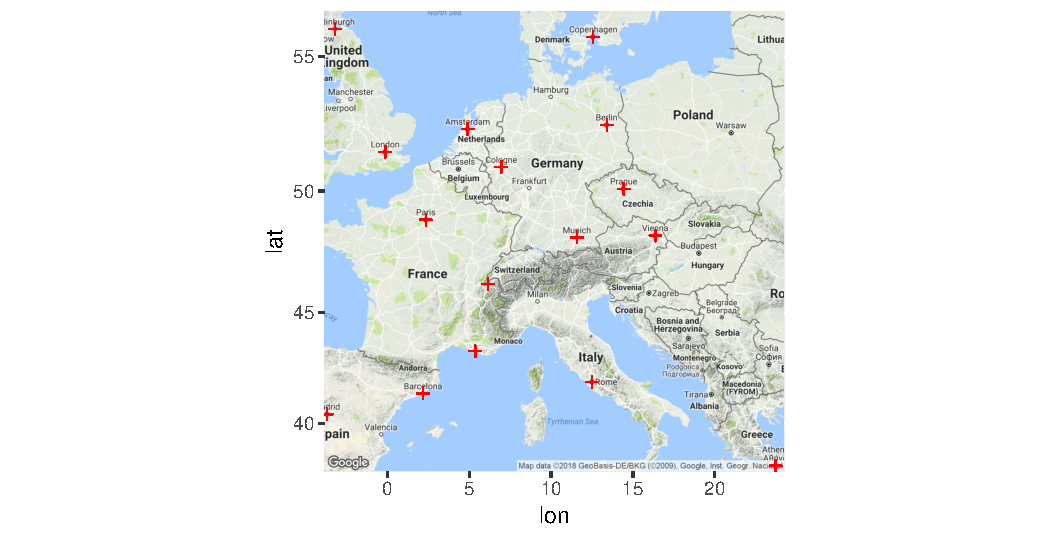
\includegraphics[width=\maxwidth]{figure/unnamed-chunk-19-1} 

\end{knitrout}
  
\end{frame}

\begin{frame}[fragile]{Reminder of data setup}

  \begin{footnotesize}
\begin{knitrout}
\definecolor{shadecolor}{rgb}{0.969, 0.969, 0.969}\color{fgcolor}\begin{kframe}
\begin{alltt}
\hlstd{miners}
\end{alltt}
\begin{verbatim}
## Source: local data frame [24 x 4]
## Groups: Exposure [8]
## 
##    Exposure Severity  Freq proportion
##       <dbl>    <chr> <int>      <dbl>
## 1       5.8     None    98 1.00000000
## 2      15.0     None    51 0.94444444
## 3      21.5     None    34 0.79069767
## 4      27.5     None    35 0.72916667
## 5      33.5     None    32 0.62745098
## 6      39.5     None    23 0.60526316
## 7      46.0     None    12 0.42857143
## 8      51.5     None     4 0.36363636
## 9       5.8 Moderate     0 0.00000000
## 10     15.0 Moderate     2 0.03703704
## # ... with 14 more rows
\end{verbatim}
\end{kframe}
\end{knitrout}
  \end{footnotesize}
\end{frame}


\begin{frame}[fragile]{Creating an ordered factor}
  
  \begin{itemize}
  \item Problem: on plot, \texttt{Severity} categories in \emph{wrong
      order}. 
  \item First we need the different values in  (text) \texttt{Severity}:
    
\begin{knitrout}
\definecolor{shadecolor}{rgb}{0.969, 0.969, 0.969}\color{fgcolor}\begin{kframe}
\begin{alltt}
\hlstd{v}\hlkwb{=}\hlkwd{unique}\hlstd{(miners}\hlopt{$}\hlstd{Severity)}
\hlstd{v}
\end{alltt}
\begin{verbatim}
## [1] "None"     "Moderate" "Severe"
\end{verbatim}
\end{kframe}
\end{knitrout}

\item These are in the right order. Now we make an ordered factor out
  of \texttt{Severity} with these as its levels. Note how it prints out:
  
  {\small
\begin{knitrout}
\definecolor{shadecolor}{rgb}{0.969, 0.969, 0.969}\color{fgcolor}\begin{kframe}
\begin{alltt}
\hlstd{severity.ord}\hlkwb{=}\hlkwd{ordered}\hlstd{(miners}\hlopt{$}\hlstd{Severity,v)}
\hlstd{severity.ord}
\end{alltt}
\begin{verbatim}
##  [1] None     None     None     None     None     None     None    
##  [8] None     Moderate Moderate Moderate Moderate Moderate Moderate
## [15] Moderate Moderate Severe   Severe   Severe   Severe   Severe  
## [22] Severe   Severe   Severe  
## Levels: None < Moderate < Severe
\end{verbatim}
\end{kframe}
\end{knitrout}
}
  \end{itemize}
  
\end{frame}

\begin{frame}[fragile]{Fitting ordered logistic model}

Use function \texttt{polr} from package \texttt{MASS}. Like \texttt{glm}.

{\small
 
\begin{knitrout}
\definecolor{shadecolor}{rgb}{0.969, 0.969, 0.969}\color{fgcolor}\begin{kframe}
\begin{alltt}
\hlkwd{library}\hlstd{(MASS)}
\end{alltt}


{\ttfamily\noindent\itshape\color{messagecolor}{\#\# \\\#\# Attaching package: 'MASS'}}

{\ttfamily\noindent\itshape\color{messagecolor}{\#\# The following object is masked from 'package:dplyr':\\\#\# \\\#\#\ \ \ \  select}}\begin{alltt}
\hlstd{miners.1}\hlkwb{=}\hlkwd{polr}\hlstd{(severity.ord}\hlopt{~}\hlstd{Exposure,}\hlkwc{weights}\hlstd{=Freq,}\hlkwc{data}\hlstd{=miners)}
\end{alltt}
\end{kframe}
\end{knitrout}
}
  
\end{frame}

\begin{frame}[fragile]{Output: not very illuminating}
  
\begin{knitrout}
\definecolor{shadecolor}{rgb}{0.969, 0.969, 0.969}\color{fgcolor}\begin{kframe}
\begin{alltt}
\hlkwd{summary}\hlstd{(miners.1)}
\end{alltt}


{\ttfamily\noindent\itshape\color{messagecolor}{\#\# \\\#\# Re-fitting to get Hessian}}\begin{verbatim}
## Call:
## polr(formula = severity.ord ~ Exposure, data = miners, weights = Freq)
## 
## Coefficients:
##           Value Std. Error t value
## Exposure 0.0959    0.01194   8.034
## 
## Intercepts:
##                 Value   Std. Error t value
## None|Moderate    3.9558  0.4097     9.6558
## Moderate|Severe  4.8690  0.4411    11.0383
## 
## Residual Deviance: 416.9188 
## AIC: 422.9188
\end{verbatim}
\end{kframe}
\end{knitrout}
  
\end{frame}
 
\begin{frame}[fragile]{Does exposure have an effect?}
  
  Fit model without \texttt{Exposure}, and compare
using \texttt{anova}. Note \texttt{1} for model with just intercept:

{\small
\begin{knitrout}
\definecolor{shadecolor}{rgb}{0.969, 0.969, 0.969}\color{fgcolor}\begin{kframe}
\begin{alltt}
\hlstd{miners.0}\hlkwb{=}\hlkwd{polr}\hlstd{(severity.ord}\hlopt{~}\hlnum{1}\hlstd{,}\hlkwc{weights}\hlstd{=Freq,}\hlkwc{data}\hlstd{=miners)}
\hlkwd{anova}\hlstd{(miners.0,miners.1)}
\end{alltt}
\begin{verbatim}
## Likelihood ratio tests of ordinal regression models
## 
## Response: severity.ord
##      Model Resid. df Resid. Dev   Test    Df LR stat. Pr(Chi)
## 1        1       369   505.1621                              
## 2 Exposure       368   416.9188 1 vs 2     1 88.24324       0
\end{verbatim}
\end{kframe}
\end{knitrout}
} 


Exposure definitely has effect on severity of disease. 

  
\end{frame}

\begin{frame}[fragile]{Predicted probabilities}

Make new data frame out of all the exposure values (from original data
frame), and predict from that:

 
\begin{knitrout}
\definecolor{shadecolor}{rgb}{0.969, 0.969, 0.969}\color{fgcolor}\begin{kframe}
\begin{alltt}
\hlstd{miners.new}\hlkwb{=}\hlkwd{data.frame}\hlstd{(}\hlkwc{Exposure}\hlstd{=freqs}\hlopt{$}\hlstd{Exposure)}
\hlstd{pr}\hlkwb{=}\hlkwd{predict}\hlstd{(miners.1,miners.new,}\hlkwc{type}\hlstd{=}\hlstr{"p"}\hlstd{)}
\hlstd{miners.pred}\hlkwb{=}\hlkwd{cbind}\hlstd{(miners.new,pr)}
\hlstd{miners.pred}
\end{alltt}
\begin{verbatim}
##   Exposure      None   Moderate     Severe
## 1      5.8 0.9676920 0.01908912 0.01321885
## 2     15.0 0.9253445 0.04329931 0.03135614
## 3     21.5 0.8692003 0.07385858 0.05694115
## 4     27.5 0.7889290 0.11413004 0.09694093
## 5     33.5 0.6776641 0.16207145 0.16026444
## 6     39.5 0.5418105 0.20484198 0.25334756
## 7     46.0 0.3879962 0.22441555 0.38758828
## 8     51.5 0.2722543 0.21025011 0.51749563
\end{verbatim}
\end{kframe}
\end{knitrout}
 
  
\end{frame}


\begin{frame}[fragile]{Comments}
  
  \begin{itemize}
  \item Model appears to match data: as exposure goes up, prob of None
    goes down, Severe goes up (sharply for high exposure).
  \item Like original data frame, this one nice to look at but
    \emph{not tidy}. We want to make graph, so tidy:
  \item Usual \texttt{gather}:
    
\begin{knitrout}
\definecolor{shadecolor}{rgb}{0.969, 0.969, 0.969}\color{fgcolor}\begin{kframe}
\begin{alltt}
\hlstd{miners.pred} \hlopt
  \hlkwd{gather}\hlstd{(Severity,probability,None}\hlopt{:}\hlstd{Severe)} \hlkwb{->} \hlstd{preds}
\hlkwd{head}\hlstd{(preds)}
\end{alltt}
\begin{verbatim}
##   Exposure Severity probability
## 1      5.8     None   0.9676920
## 2     15.0     None   0.9253445
## 3     21.5     None   0.8692003
## 4     27.5     None   0.7889290
## 5     33.5     None   0.6776641
## 6     39.5     None   0.5418105
\end{verbatim}
\end{kframe}
\end{knitrout}

  \end{itemize}
  
\end{frame}

\begin{frame}[fragile]{Plotting predicted and observed proportions}
  
  Plot:
  \begin{itemize}
  \item predicted probabilities, lines (shown) joining points (not shown)
  \item data, just the points. 
  
  Unfamiliar process: data from two \emph{different} data frames:
  
\begin{knitrout}
\definecolor{shadecolor}{rgb}{0.969, 0.969, 0.969}\color{fgcolor}\begin{kframe}
\begin{alltt}
\hlstd{g}\hlkwb{=}\hlkwd{ggplot}\hlstd{(preds,}\hlkwd{aes}\hlstd{(}\hlkwc{x}\hlstd{=Exposure,}\hlkwc{y}\hlstd{=probability,}
    \hlkwc{colour}\hlstd{=Severity))}\hlopt{+}
  \hlkwd{geom_line}\hlstd{()}\hlopt{+}
  \hlkwd{geom_point}\hlstd{(}\hlkwc{data}\hlstd{=miners,}\hlkwd{aes}\hlstd{(}\hlkwc{y}\hlstd{=proportion))}
\end{alltt}
\end{kframe}
\end{knitrout}

\item Idea: final \texttt{geom\_point} uses data in \texttt{miners}
  rather than \texttt{preds}, $y$-variable for plot is \texttt{prop}
  from that data frame, but $x$-coordinate is \texttt{Exposure}, as it
  was before, and \texttt{colour} is \texttt{Severity} as before. The
  final \texttt{geom\_point} ``inherits'' from the first \texttt{aes}
  as needed.
\item Data conform to fitted relationship pretty well:
  \end{itemize}
  
\end{frame}

\begin{frame}[fragile]{The plot}
  
\begin{knitrout}
\definecolor{shadecolor}{rgb}{0.969, 0.969, 0.969}\color{fgcolor}\begin{kframe}
\begin{alltt}
\hlstd{g}
\end{alltt}
\end{kframe}
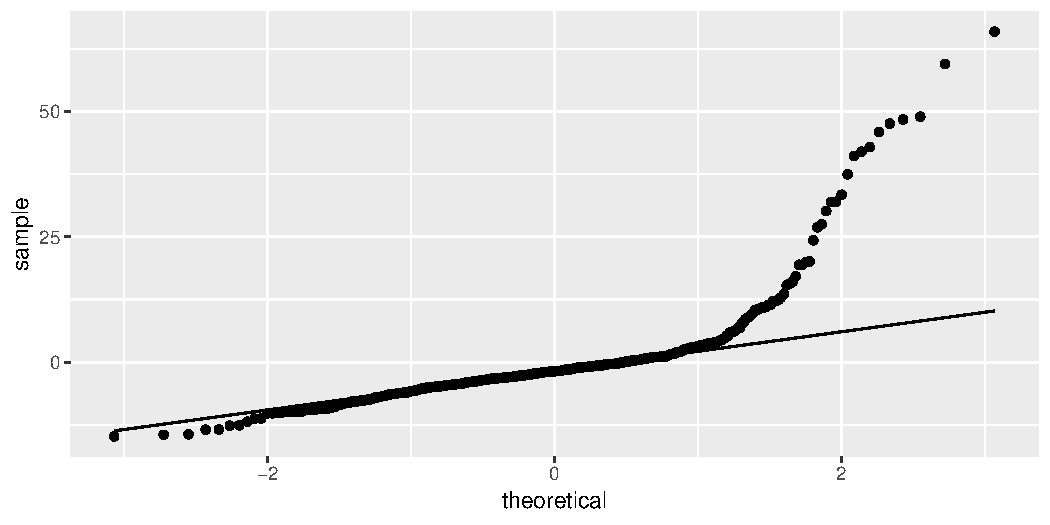
\includegraphics[width=\maxwidth]{figure/unnamed-chunk-29-1} 

\end{knitrout}
  
\end{frame}




% mlogit.pdf

\begin{frame}[fragile]{Unordered responses}

  \begin{itemize}
  \item With unordered (nominal) responses, can use {\em generalized logit}.
  \item Example: 735 people, record age and sex (male 0, female 1), which of 3 brands of some product preferred.
  \item Data in \verb-mlogit.csv- separated by commas (so
    \texttt{read.csv} will work):

 
\begin{knitrout}
\definecolor{shadecolor}{rgb}{0.969, 0.969, 0.969}\color{fgcolor}\begin{kframe}
\begin{alltt}
\hlstd{brandpref}\hlkwb{=}\hlkwd{read.csv}\hlstd{(}\hlstr{"mlogit.csv"}\hlstd{,}\hlkwc{header}\hlstd{=T)}
\hlkwd{head}\hlstd{(brandpref)}
\end{alltt}
\begin{verbatim}
##   brand sex age
## 1     1   0  24
## 2     1   0  26
## 3     1   0  26
## 4     1   1  27
## 5     1   1  27
## 6     3   1  27
\end{verbatim}
\end{kframe}
\end{knitrout}
    

  \end{itemize}

\end{frame}

\begin{frame}[fragile]{Bashing into shape, and fitting model}

  \begin{itemize}
  \item \texttt{sex} and \texttt{brand} not meaningful as numbers, so
    turn into factors
 
\begin{knitrout}
\definecolor{shadecolor}{rgb}{0.969, 0.969, 0.969}\color{fgcolor}\begin{kframe}
\begin{alltt}
\hlstd{brandpref}\hlopt{$}\hlstd{sex}\hlkwb{=}\hlkwd{factor}\hlstd{(brandpref}\hlopt{$}\hlstd{sex)}
\hlstd{brandpref}\hlopt{$}\hlstd{brand}\hlkwb{=}\hlkwd{factor}\hlstd{(brandpref}\hlopt{$}\hlstd{brand)}
\end{alltt}
\end{kframe}
\end{knitrout}
    
  \item We use \texttt{multinom} from package \texttt{nnet}. Works
    like \texttt{polr}.
  \end{itemize}

 
\begin{knitrout}
\definecolor{shadecolor}{rgb}{0.969, 0.969, 0.969}\color{fgcolor}\begin{kframe}
\begin{alltt}
\hlkwd{library}\hlstd{(nnet)}
\hlstd{brands.both}\hlkwb{=}\hlkwd{multinom}\hlstd{(brand}\hlopt{~}\hlstd{age}\hlopt{+}\hlstd{sex,}\hlkwc{data}\hlstd{=brandpref)}
\end{alltt}
\begin{verbatim}
## # weights:  12 (6 variable)
## initial  value 807.480032 
## iter  10 value 702.976983
## final  value 702.970704 
## converged
\end{verbatim}
\end{kframe}
\end{knitrout}
  
\end{frame}

\begin{frame}[fragile]{Do age/sex help predict brand? 1/2}

Fit models without each:

 
\begin{knitrout}
\definecolor{shadecolor}{rgb}{0.969, 0.969, 0.969}\color{fgcolor}\begin{kframe}
\begin{alltt}
\hlstd{brands.age}\hlkwb{=}\hlkwd{multinom}\hlstd{(brand}\hlopt{~}\hlstd{age,}\hlkwc{data}\hlstd{=brandpref)}
\end{alltt}
\begin{verbatim}
## # weights:  9 (4 variable)
## initial  value 807.480032 
## iter  10 value 706.796323
## iter  10 value 706.796322
## final  value 706.796322 
## converged
\end{verbatim}
\begin{alltt}
\hlstd{brands.sex}\hlkwb{=}\hlkwd{multinom}\hlstd{(brand}\hlopt{~}\hlstd{sex,}\hlkwc{data}\hlstd{=brandpref)}
\end{alltt}
\begin{verbatim}
## # weights:  9 (4 variable)
## initial  value 807.480032 
## final  value 791.861266 
## converged
\end{verbatim}
\end{kframe}
\end{knitrout}


  
\end{frame}

\begin{frame}[fragile]{Do age/sex help predict brand? 2/2}

{\footnotesize  
 
\begin{knitrout}
\definecolor{shadecolor}{rgb}{0.969, 0.969, 0.969}\color{fgcolor}\begin{kframe}
\begin{alltt}
\hlkwd{anova}\hlstd{(brands.age,brands.both)}
\end{alltt}
\begin{verbatim}
## Likelihood ratio tests of Multinomial Models
## 
## Response: brand
##       Model Resid. df Resid. Dev   Test    Df LR stat.    Pr(Chi)
## 1       age      1466   1413.593                                 
## 2 age + sex      1464   1405.941 1 vs 2     2 7.651236 0.02180495
\end{verbatim}
\begin{alltt}
\hlkwd{anova}\hlstd{(brands.sex,brands.both)}
\end{alltt}
\begin{verbatim}
## Likelihood ratio tests of Multinomial Models
## 
## Response: brand
##       Model Resid. df Resid. Dev   Test    Df LR stat. Pr(Chi)
## 1       sex      1466   1583.723                              
## 2 age + sex      1464   1405.941 1 vs 2     2 177.7811       0
\end{verbatim}
\end{kframe}
\end{knitrout}
  }
  
\begin{itemize}
\item \texttt{age} definitely significant (second \texttt{anova})
\item \texttt{sex} seems significant also (first \texttt{anova})
\item Keep both.
\end{itemize}
  
  
\end{frame}

\begin{frame}[fragile]{Another way to build model}
  
  \begin{itemize}
  \item Start from model with everything and feed into \texttt{step}:
    
    {\small
\begin{knitrout}
\definecolor{shadecolor}{rgb}{0.969, 0.969, 0.969}\color{fgcolor}\begin{kframe}
\begin{alltt}
\hlkwd{step}\hlstd{(brands.both,}\hlkwc{trace}\hlstd{=}\hlnum{0}\hlstd{)}
\end{alltt}
\begin{verbatim}
## trying - age 
## trying - sex
## Call:
## multinom(formula = brand ~ age + sex, data = brandpref)
## 
## Coefficients:
##   (Intercept)       age      sex1
## 2   -11.77469 0.3682075 0.5238197
## 3   -22.72141 0.6859087 0.4659488
## 
## Residual Deviance: 1405.941 
## AIC: 1417.941
\end{verbatim}
\end{kframe}
\end{knitrout}
}

\item Final model contains both \texttt{age} and \texttt{sex} so neither
could be removed.
  \end{itemize}
  
\end{frame}

\begin{frame}[fragile]{Predictions}

Create data frame with various age and sex. Feed into \texttt{predict}.

{\footnotesize
 
\begin{knitrout}
\definecolor{shadecolor}{rgb}{0.969, 0.969, 0.969}\color{fgcolor}\begin{kframe}
\begin{alltt}
\hlstd{new}\hlkwb{=}\hlkwd{expand.grid}\hlstd{(}\hlkwc{age}\hlstd{=}\hlkwd{c}\hlstd{(}\hlnum{24}\hlstd{,}\hlnum{28}\hlstd{,}\hlnum{32}\hlstd{,}\hlnum{35}\hlstd{,}\hlnum{38}\hlstd{),}\hlkwc{sex}\hlstd{=}\hlkwd{factor}\hlstd{(}\hlnum{0}\hlopt{:}\hlnum{1}\hlstd{))}
\hlstd{pr}\hlkwb{=}\hlkwd{predict}\hlstd{(brands.both,new,}\hlkwc{type}\hlstd{=}\hlstr{"probs"}\hlstd{)}
\hlstd{probs}\hlkwb{=}\hlkwd{cbind}\hlstd{(new,pr)}
\hlstd{probs}
\end{alltt}
\begin{verbatim}
##    age sex          1          2           3
## 1   24   0 0.94795822 0.05022928 0.001812497
## 2   28   0 0.79313204 0.18329690 0.023571058
## 3   32   0 0.40487271 0.40810321 0.187024082
## 4   35   0 0.13057819 0.39724053 0.472181272
## 5   38   0 0.02598163 0.23855071 0.735467663
## 6   24   1 0.91532076 0.08189042 0.002788820
## 7   28   1 0.69561789 0.27143910 0.032943012
## 8   32   1 0.29086347 0.49503135 0.214105181
## 9   35   1 0.08404134 0.43168592 0.484272746
## 10  38   1 0.01623089 0.25162197 0.732147148
\end{verbatim}
\end{kframe}
\end{knitrout}
}

\begin{itemize}
\item Young males (\texttt{sex=0}) prefer brand 1, 
but older males prefer brand 3.
\item Females similar, but like brand 1 less and
  brand 2 more.
\end{itemize}

\end{frame}

\begin{frame}[fragile]{Making a plot}
  
  \begin{itemize}
  \item Plot fitted probability against age, distinguishing brand by
    colour and gender by plotting symbol.
  \item Also join points by lines, and distinguish lines by gender. 
  \item I thought about facetting, but this seems to come out clearer.
  \item First need tidy data frame, by familiar process:
    
\begin{knitrout}
\definecolor{shadecolor}{rgb}{0.969, 0.969, 0.969}\color{fgcolor}\begin{kframe}
\begin{alltt}
\hlstd{probs} \hlopt \hlkwd{gather}\hlstd{(brand,probability,}\hlopt{-}\hlstd{(age}\hlopt{:}\hlstd{sex))} \hlkwb{->} \hlstd{probs.long}
\hlkwd{sample_n}\hlstd{(probs.long,}\hlnum{7}\hlstd{)}
\end{alltt}
\begin{verbatim}
##    age sex brand probability
## 2   28   0     1  0.79313204
## 24  35   0     3  0.47218127
## 27  28   1     3  0.03294301
## 13  32   0     2  0.40810321
## 25  38   0     3  0.73546766
## 7   28   1     1  0.69561789
## 12  28   0     2  0.18329690
\end{verbatim}
\end{kframe}
\end{knitrout}
\item Then (over):
  
  \end{itemize}
  
\end{frame}

\begin{frame}[fragile]{The plot}
  
\begin{knitrout}
\definecolor{shadecolor}{rgb}{0.969, 0.969, 0.969}\color{fgcolor}\begin{kframe}
\begin{alltt}
\hlkwd{ggplot}\hlstd{(probs.long,}\hlkwd{aes}\hlstd{(}\hlkwc{x}\hlstd{=age,}\hlkwc{y}\hlstd{=probability,}
  \hlkwc{colour}\hlstd{=brand,}\hlkwc{shape}\hlstd{=sex))}\hlopt{+}
  \hlkwd{geom_point}\hlstd{()}\hlopt{+}\hlkwd{geom_line}\hlstd{(}\hlkwd{aes}\hlstd{(}\hlkwc{linetype}\hlstd{=sex))}
\end{alltt}
\end{kframe}
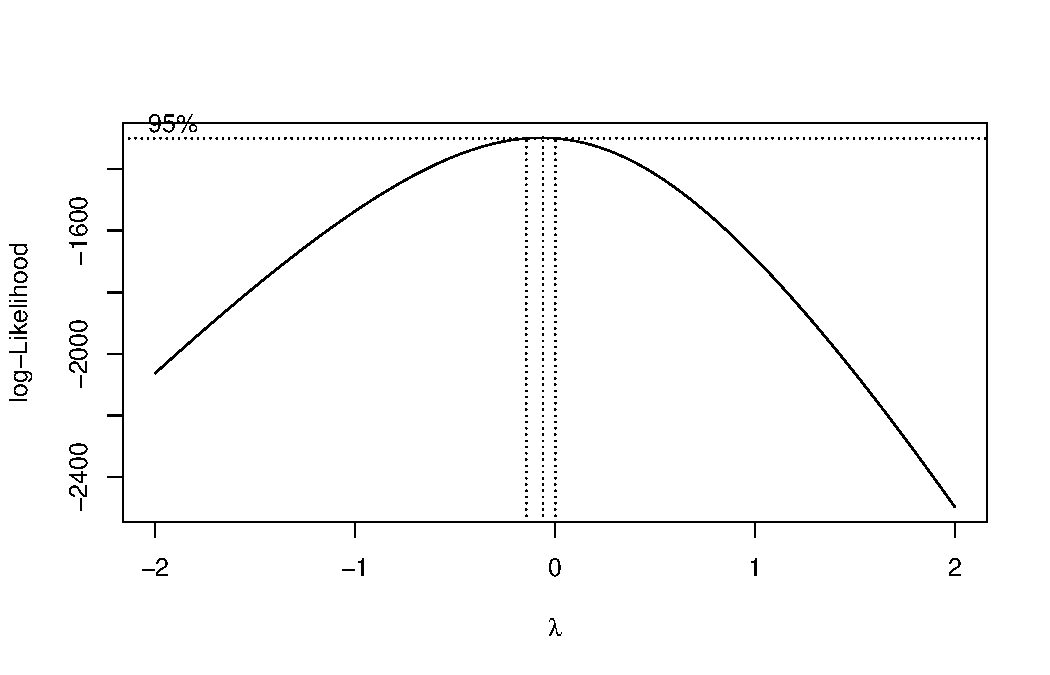
\includegraphics[width=\maxwidth]{figure/unnamed-chunk-38-1} 

\end{knitrout}
\end{frame}


\begin{frame}[fragile]{Digesting the plot}
  
  \begin{itemize}
  \item Brand vs.\ age: younger people (of both genders) prefer brand
    1, but older people (of both genders) prefer brand 3. (Explains
    significant age effect.)
  \item Brand vs.\ sex: females (dashed) like brand 1 less than males
    (solid), like brand 2 more (for all ages). 
    more.
  \item Not much brand difference between genders (solid and dashed
    lines of same colours close), but enough to be significant.
  \item Model didn't include interaction, so modelled effect of gender
    on brand same for each age, modelled effect of age same for each
    gender. 
  \end{itemize}
  
\end{frame}


\begin{frame}[fragile]{Alternative data format}

Summarize all people of same brand preference, same sex, same age on one line of data file with frequency on end:

{
\begin{verbatim}
1 0 24 1
1 0 26 2
1 0 27 4
1 0 28 4
1 0 29 7
1 0 30 3
...
\end{verbatim}
}

Whole data set in 65 lines not 735! But how?
  
\end{frame}

\begin{frame}[fragile]{Getting alternative data format}
  
\begin{knitrout}
\definecolor{shadecolor}{rgb}{0.969, 0.969, 0.969}\color{fgcolor}\begin{kframe}
\begin{alltt}
\hlstd{brandpref} \hlopt
  \hlkwd{group_by}\hlstd{(age,sex,brand)} \hlopt
  \hlkwd{summarize}\hlstd{(}\hlkwc{Freq}\hlstd{=}\hlkwd{n}\hlstd{())} \hlkwb{->} \hlstd{b}
\hlkwd{head}\hlstd{(b)}
\end{alltt}
\begin{verbatim}
## Source: local data frame [6 x 4]
## Groups: age, sex [5]
## 
##     age    sex  brand  Freq
##   <int> <fctr> <fctr> <int>
## 1    24      0      1     1
## 2    26      0      1     2
## 3    27      0      1     4
## 4    27      1      1     4
## 5    27      1      3     1
## 6    28      0      1     4
\end{verbatim}
\end{kframe}
\end{knitrout}
  
\end{frame}



\begin{frame}[fragile]{Fitting models, almost the same}

  \begin{itemize}
  \item Just have to remember \texttt{weights} to incorporate
frequencies.
\item Otherwise \texttt{multinom} assumes you have just 1 obs
on each line!
\item Again turn (numerical) \texttt{sex} and \texttt{brand} into factors:
{\small
 
\begin{knitrout}
\definecolor{shadecolor}{rgb}{0.969, 0.969, 0.969}\color{fgcolor}\begin{kframe}
\begin{alltt}
\hlstd{b}\hlopt{$}\hlstd{sex}\hlkwb{=}\hlkwd{factor}\hlstd{(b}\hlopt{$}\hlstd{sex)}
\hlstd{b}\hlopt{$}\hlstd{brand}\hlkwb{=}\hlkwd{factor}\hlstd{(b}\hlopt{$}\hlstd{brand)}
\hlstd{b.both}\hlkwb{=}\hlkwd{multinom}\hlstd{(brand}\hlopt{~}\hlstd{age}\hlopt{+}\hlstd{sex,}\hlkwc{data}\hlstd{=b,}\hlkwc{weights}\hlstd{=Freq)}
\end{alltt}
\begin{verbatim}
## # weights:  12 (6 variable)
## initial  value 807.480032 
## iter  10 value 702.976983
## final  value 702.970704 
## converged
\end{verbatim}
\begin{alltt}
\hlstd{b.age}\hlkwb{=}\hlkwd{multinom}\hlstd{(brand}\hlopt{~}\hlstd{age,}\hlkwc{data}\hlstd{=b,}\hlkwc{weights}\hlstd{=Freq)}
\end{alltt}
\begin{verbatim}
## # weights:  9 (4 variable)
## initial  value 807.480032 
## iter  10 value 706.796323
## iter  10 value 706.796322
## final  value 706.796322 
## converged
\end{verbatim}
\end{kframe}
\end{knitrout}
}  

  \end{itemize}

  
\end{frame}

\begin{frame}[fragile]{P-value for \texttt{sex} identical}
  
{\small  
 
\begin{knitrout}
\definecolor{shadecolor}{rgb}{0.969, 0.969, 0.969}\color{fgcolor}\begin{kframe}
\begin{alltt}
\hlkwd{anova}\hlstd{(b.age,b.both)}
\end{alltt}
\begin{verbatim}
## Likelihood ratio tests of Multinomial Models
## 
## Response: brand
##       Model Resid. df Resid. Dev   Test    Df LR stat.    Pr(Chi)
## 1       age       126   1413.593                                 
## 2 age + sex       124   1405.941 1 vs 2     2 7.651236 0.02180495
\end{verbatim}
\end{kframe}
\end{knitrout}
}

Same P-value as before, so we haven't changed anything important.
  
\end{frame}

\begin{frame}[fragile]{Including data on plot}
  
  \begin{itemize}
  \item Everyone's age given as whole
    number, so maybe not too many different ages with sensible amount
    of data at each:
    
    \begin{footnotesize}
\begin{knitrout}
\definecolor{shadecolor}{rgb}{0.969, 0.969, 0.969}\color{fgcolor}\begin{kframe}
\begin{alltt}
\hlstd{b} \hlopt \hlkwd{group_by}\hlstd{(age)} \hlopt
  \hlkwd{summarize}\hlstd{(}\hlkwc{total}\hlstd{=}\hlkwd{sum}\hlstd{(Freq))}
\end{alltt}
\begin{verbatim}
## # A tibble: 14 × 2
##      age total
##    <int> <int>
## 1     24     1
## 2     26     2
## 3     27     9
## 4     28    15
## 5     29    19
## 6     30    23
## 7     31    40
## 8     32   333
## 9     33    55
## 10    34    64
## 11    35    35
## 12    36    85
## 13    37    22
## 14    38    32
\end{verbatim}
\end{kframe}
\end{knitrout}
%$ %$
    \end{footnotesize}
    
   
  \end{itemize}
  
\end{frame}

\begin{frame}[fragile]{Comments and next}
  \begin{itemize}
  \item Not great (especially at low end), but live with it.
  \item Need proportions of frequencies in each brand for each
    age-gender combination. Mimic what we did for miners:
\begin{knitrout}
\definecolor{shadecolor}{rgb}{0.969, 0.969, 0.969}\color{fgcolor}\begin{kframe}
\begin{alltt}
\hlstd{b} \hlopt
  \hlkwd{group_by}\hlstd{(age,sex)} \hlopt
  \hlkwd{mutate}\hlstd{(}\hlkwc{proportion}\hlstd{=}\hlkwd{prop.table}\hlstd{(Freq))} \hlkwb{->} \hlstd{brands}
\end{alltt}
\end{kframe}
\end{knitrout}
  \end{itemize}
\end{frame}

\begin{frame}[fragile]{Checking proportions for age 32}
  
  
\begin{knitrout}
\definecolor{shadecolor}{rgb}{0.969, 0.969, 0.969}\color{fgcolor}\begin{kframe}
\begin{alltt}
\hlstd{brands} \hlopt \hlkwd{filter}\hlstd{(age}\hlopt{==}\hlnum{32}\hlstd{)}
\end{alltt}
\begin{verbatim}
## Source: local data frame [6 x 5]
## Groups: age, sex [2]
## 
##     age    sex  brand  Freq proportion
##   <int> <fctr> <fctr> <int>      <dbl>
## 1    32      0      1    48  0.4067797
## 2    32      0      2    51  0.4322034
## 3    32      0      3    19  0.1610169
## 4    32      1      1    62  0.2883721
## 5    32      1      2   117  0.5441860
## 6    32      1      3    36  0.1674419
\end{verbatim}
\end{kframe}
\end{knitrout}

\begin{itemize}
\item First three proportions (males) add up to 1.
\item Last three proportions (females) add up to 1.
\item So looks like proportions of right thing.
  
\end{itemize}
  
\end{frame}

\begin{frame}[fragile]{Attempting plot}
  
  \begin{itemize}
  \item Take code from previous plot and:
    \begin{itemize}
    \item remove \texttt{geom\_point} for fitted values
    \item add \texttt{geom\_point} with correct \texttt{data=} and
      \texttt{aes} to plot data.
    \end{itemize}
    
\begin{knitrout}
\definecolor{shadecolor}{rgb}{0.969, 0.969, 0.969}\color{fgcolor}\begin{kframe}
\begin{alltt}
\hlstd{g}\hlkwb{=}\hlkwd{ggplot}\hlstd{(probs.long,}\hlkwd{aes}\hlstd{(}\hlkwc{x}\hlstd{=age,}\hlkwc{y}\hlstd{=probability,}
  \hlkwc{colour}\hlstd{=brand,}\hlkwc{shape}\hlstd{=sex))}\hlopt{+}
  \hlkwd{geom_line}\hlstd{(}\hlkwd{aes}\hlstd{(}\hlkwc{linetype}\hlstd{=sex))}\hlopt{+}
  \hlkwd{geom_point}\hlstd{(}\hlkwc{data}\hlstd{=brands,}\hlkwd{aes}\hlstd{(}\hlkwc{y}\hlstd{=proportion))}
\end{alltt}
\end{kframe}
\end{knitrout}

\item Data seem to correspond more or less to fitted curves:
  \end{itemize}
  
\end{frame}

\begin{frame}[fragile]{The plot}
  
\begin{knitrout}
\definecolor{shadecolor}{rgb}{0.969, 0.969, 0.969}\color{fgcolor}\begin{kframe}
\begin{alltt}
\hlstd{g}
\end{alltt}
\end{kframe}
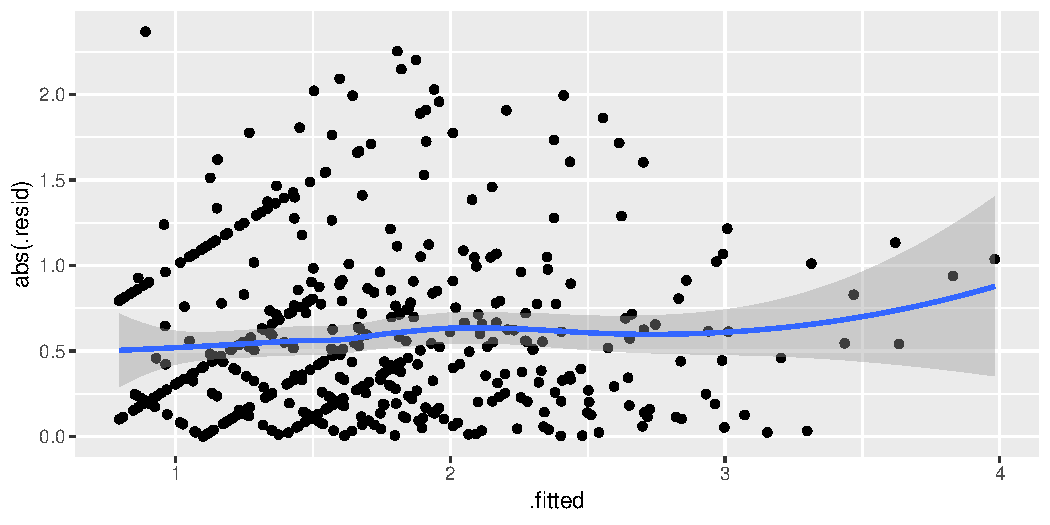
\includegraphics[width=\maxwidth]{figure/unnamed-chunk-45-1} 

\end{knitrout}
\end{frame}

\begin{frame}[fragile]{Trying interaction between age and gender}
  
  \begin{scriptsize}
\begin{knitrout}
\definecolor{shadecolor}{rgb}{0.969, 0.969, 0.969}\color{fgcolor}\begin{kframe}
\begin{alltt}
\hlstd{b.int}\hlkwb{=}\hlkwd{update}\hlstd{(b.both,.}\hlopt{~}\hlstd{.}\hlopt{+}\hlstd{age}\hlopt{:}\hlstd{sex)}
\end{alltt}
\begin{verbatim}
## # weights:  15 (8 variable)
## initial  value 807.480032 
## iter  10 value 704.811229
## iter  20 value 702.582802
## final  value 702.582761 
## converged
\end{verbatim}
\begin{alltt}
\hlkwd{anova}\hlstd{(b.both,b.int)}
\end{alltt}
\begin{verbatim}
## Likelihood ratio tests of Multinomial Models
## 
## Response: brand
##                 Model Resid. df Resid. Dev   Test    Df  LR stat.  Pr(Chi)
## 1           age + sex       124   1405.941                                
## 2 age + sex + age:sex       122   1405.166 1 vs 2     2 0.7758861 0.678451
\end{verbatim}
\end{kframe}
\end{knitrout}
    
  \end{scriptsize}

  \begin{itemize}
  \item No evidence that effect of age on brand preference differs for
    the two genders.
  \end{itemize}
\end{frame}
